\documentclass[twoside,10pt]{article}
\usepackage{/Users/bradenhoagland/latex/styles/toggles}
%\toggletrue{sectionbreaks}
%\toggletrue{sectionheaders}
\newcommand{\docTitle}{HW 2}
\usepackage{/Users/bradenhoagland/latex/styles/common}
\importStyles{modern}{rainbow}{boxy}

%\renewcommand{\theenumi}{\alph{enumi}}

\begin{document}
%\tableofcontents

% ------------------------------
% 1.29
% ------------------------------
\begin{exer}[1.29]
Bow Tie Lemma.
\end{exer}

Both angles subtend the same arc $BC$, so they are both equal to $\frac{1}{2} \angle BOC$ by the Star Trek lemma.

\newpage

% ------------------------------
% 1.43
% ------------------------------
\begin{exer}[1.43]
The Angle Bisector Theorem.
\end{exer}

\begin{figure}[H]
	\centering
	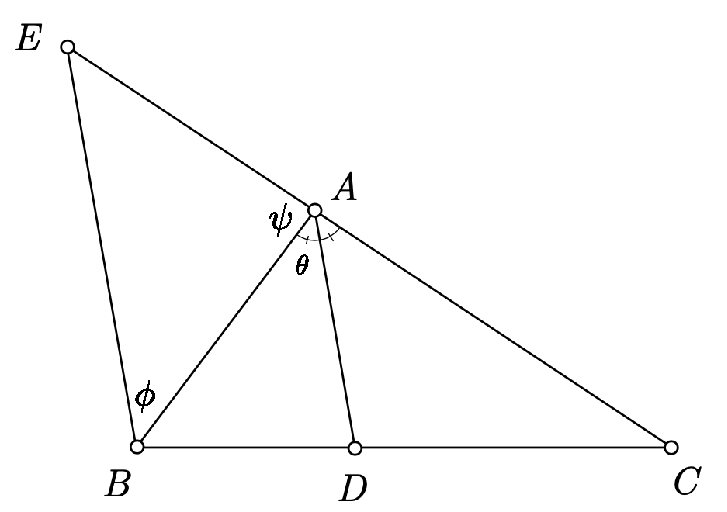
\includegraphics[scale=0.7]{fig/43.pdf}
\end{figure}


Construct the line $\ell_1$ parallel to $AD$ and going through $B$. Since $AD$ and $AC$ are not parallel, $\ell_1$ intersects $AC$ eventually. Call this intersection point $E$. Then by theorem 1.7.2,
\[
	\frac{|EC|}{|AC|} = \frac{|DC|}{|BC|} .
\] Now note that the angles $\theta$ and $\phi_1$ are opposite interior angles, so $\theta=\phi$. The angle $\psi$ is then equal to $180\degree -2\theta = 180\degree -2\phi$, so the last unmarked angle in triangle $\Delta EAB$ is also $\phi$. This means $\Delta EAB$ is an isosceles triangle, i.e. $|AE|=|AB|$.

Because of this, $|EC| = |EA|+|AC| = |AB|+|AC|$. Since $|BC| = |BD|+|DC|$, we can combine this with our earlier equivalent ratios to get
\[
\frac{|AB|+|AC|}{|AC|} = \frac{|BD|+|DC|}{|DC|} \implies \frac{|AB|}{|AC|} = \frac{|BD|}{|DC|} .
\] 

\newpage

% ------------------------------
% 1.49
% ------------------------------
\begin{exer}[1.49]
Show that $|CD|$ is independent of the choice of $P$.
\end{exer}

\begin{figure}[H]
	\centering
	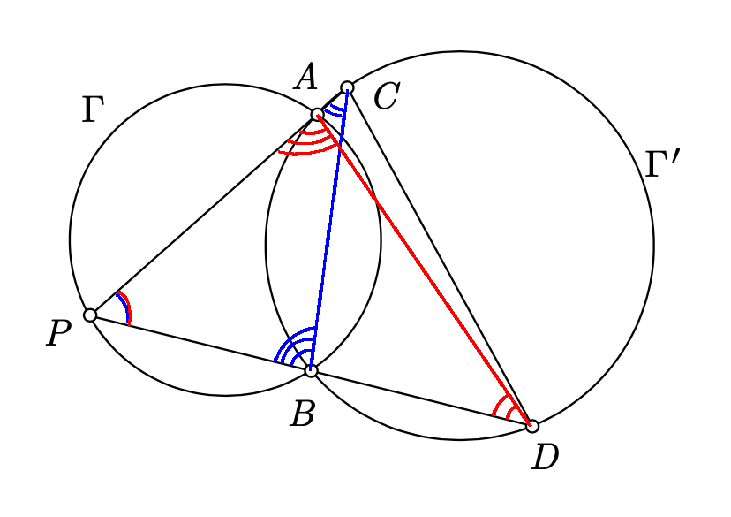
\includegraphics[scale=0.6]{fig/49.pdf}
	%\caption{}
\end{figure}

\textbf{Case 1:} Note that ${\color{blue}\angle CPB} = {\color{red}\angle APD}$ must always pass through both $A$ and $B$, which never change. Thus by the Star Trek lemma, ${\color{blue}\angle CPB}={\color{red}\angle APD}$ is constant when $P$ is changed. Similarly, ${\color{blue}\angle ACB} = {\color{red}\angle ADB}$ are also both constant.

Note that both pairs of angles are in triangles ${\color{blue}\Delta PCB}$ and ${\color{red}\Delta PAD}$, respectively, which implies that ${\color{blue}\angle PBC} = {\color{red}\angle PAD}$ are both constant. This in turn implies $\angle CAD = \angle CBD$ are both constant. Since these both subtend the arc $CD$, this means $|CD|$ is constant.

\begin{figure}[H]
	\centering
	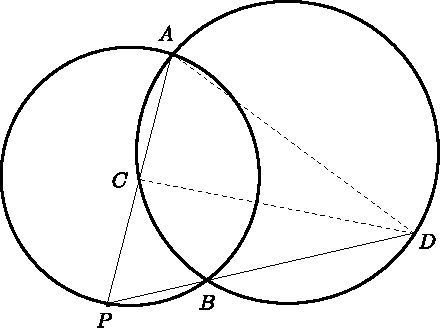
\includegraphics[scale=0.8]{fig/49-2.pdf}
	%\caption{}
\end{figure}

\textbf{Case 2:} Without loss of generality, we consider just the case when $C$ lies on $AP$, as the case when $D$ lies on $PB$ is symmetric. By a similar argument as in case 1, $\angle APD, \angle ADP$ are constant. Thus $\angle PAD = \angle CAD$, as the last angle in $\Delta PAD$, is also constant. But this subtends the arc $CD$, so $|CD|$ is constant.


\newpage

% ------------------------------
% 1.52
% ------------------------------
\begin{exer}[1.52]
What is $|DE|$?
\end{exer}

\begin{figure}[H]
	\centering
	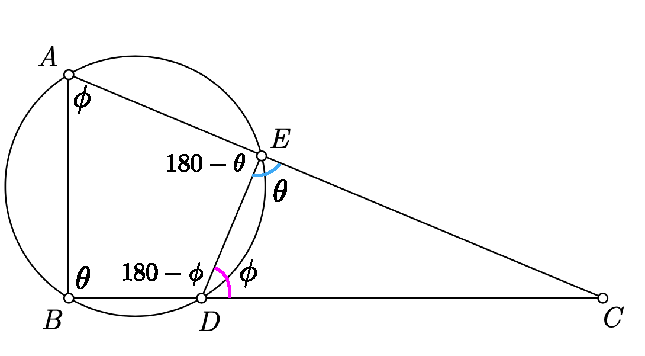
\includegraphics[scale=0.8]{fig/52.pdf}
\end{figure}

By the Star Trek theorem, since opposing angles of $AEDB$ subtend disjoint arcs that span the whole circle, the opposing angles are supplementary. This implies that the blue angle is $\theta$ and the pink angle is $\phi$. This further implies that $\Delta DEC \sim \Delta ABC$, which gives the ratio
\[
\frac{|DE|}{|AB|} = \frac{|DC|}{|AC|} \implies \frac{|DE|}{5} = \frac{9}{13} \implies |DE| = \frac{45}{13} .
\] 

\newpage

% ------------------------------
% 1.53
% ------------------------------
\begin{exer}[1.53]
Tangential version of Power of the Point.
\end{exer}

\begin{figure}[H]
	\centering
	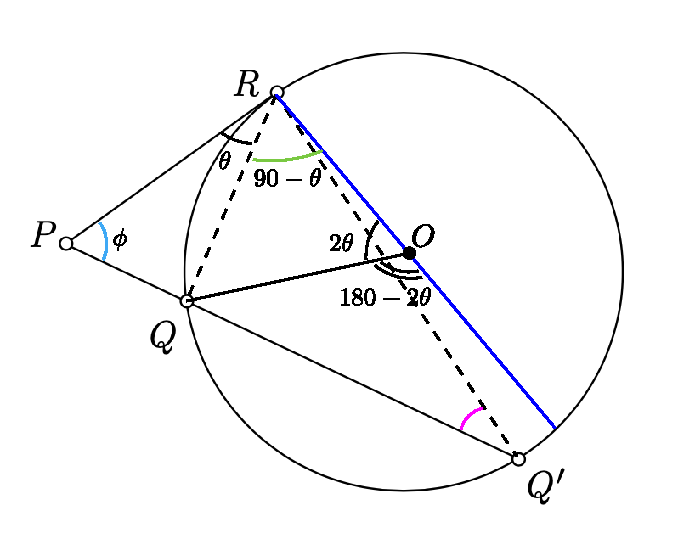
\includegraphics[scale=0.7]{fig/53.pdf}
\end{figure}

Draw the diameter through $R$ and the origin $O$. Since $PR$ is tangent to the circle, it forms a right angle with this diameter. Thus the pictured angle $\theta$ is complimentary to the green angle. Then by the Star Trek lemma, $\angle QOQ' = 180\degree -2\theta$. The adjacent angle to this, since it's a long a line, is then just $2\theta$. Applying the Star Trek lemma again, the pink angle $\angle QQ'R = \theta$.

Note that $\Delta PQR$ and $\Delta PRQ'$ already share the blue angle $\phi$, so they're similar. This gives the ratio
\[
\frac{|PR|}{|PQ'|} = \frac{|PQ|}{|PR|} \implies |PR|^2 = |PQ| \; |PQ'|.
\] 

\newpage

% ------------------------------
% 1.54
% ------------------------------
\begin{exer}[1.54]
	Use the tangential power of the point to prove the Pythagorean Theorem.
\end{exer}

\begin{figure}[H]
	\centering
	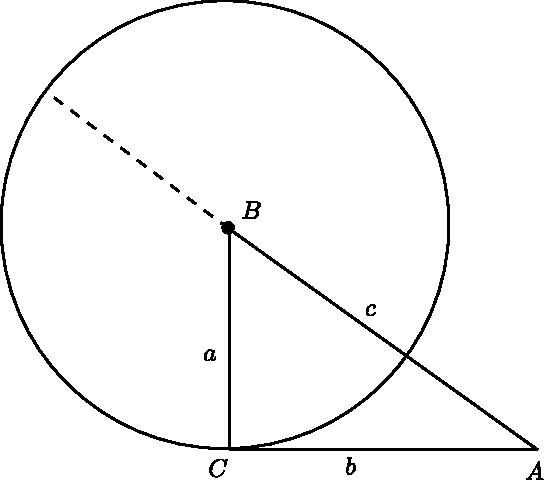
\includegraphics[scale=0.7]{fig/54.pdf}
	%\caption{}
\end{figure}

Fix the right triangle $BAC$, then construct the circle of radius $a$ with center $B$. Since $\angle BCA=90\degree$, the line segement $CA$ is tangent to the circle. Suppose the line extending $AB$ intersects the circle as pictured, then by the tangential version of power of the point,
\begin{align*}
	b^2 &= (c-a)(c+a) \\
	b^2 &= c^2-a^2,
\end{align*}
which implies $a^2+b^2=c^2$.

\newpage

% ------------------------------
% 1.57
% ------------------------------
\begin{exer}[1.57]
Find the side lengths of the triangle $\Delta ABC$.
\end{exer}

\begin{figure}[H]
	\centering
	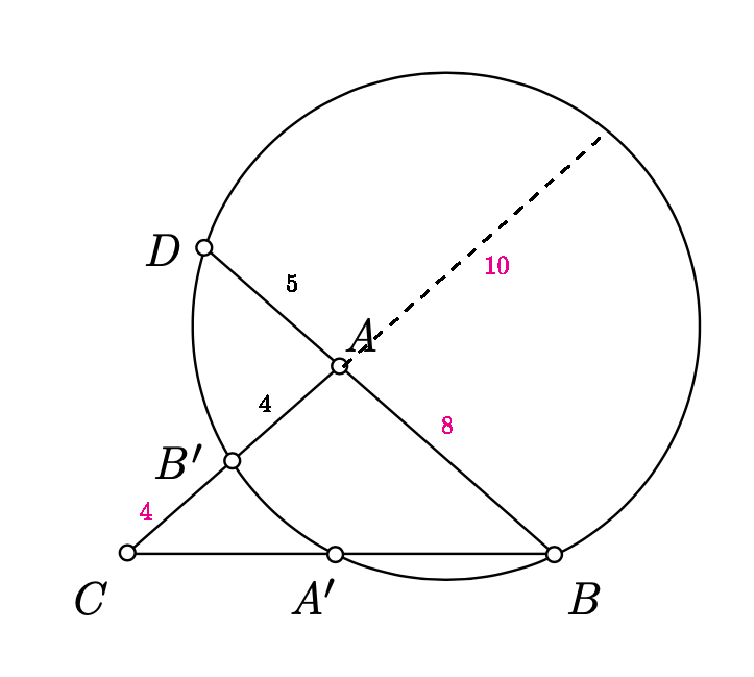
\includegraphics[scale=0.6]{fig/57.pdf}
	%\caption{}
\end{figure}

Since $|AB'|=4$, $B'$ is the midpoint of $ AC$, and $|AC|=|AB|$, we know $|AB|=|AC|=8$ and $|CB'|=4$. Then by the power of the point (inside the circle), the dashed line has length $d$ satisfying $5 \cdot 8 = 4d$, i.e. $d=10$.

Then by the power of the point again (outside the circle), $18 \cdot 4 = |CA'|\;|CB| = 2 |CA'|^2$, where the last equality follows from $A'$ being a midpoint of $CB$. This implies $|CA'|=6$, so $|CB|=12$.

Thus the two equal sides of the triangle are length 8, and the base is length 12.

\newpage

\end{document}
